\documentclass[1p]{elsarticle_modified}
%\bibliographystyle{elsarticle-num}

%\usepackage[colorlinks]{hyperref}
%\usepackage{abbrmath_seonhwa} %\Abb, \Ascr, \Acal ,\Abf, \Afrak
\usepackage{amsfonts}
\usepackage{amssymb}
\usepackage{amsmath}
\usepackage{amsthm}
\usepackage{scalefnt}
\usepackage{amsbsy}
\usepackage{kotex}
\usepackage{caption}
\usepackage{subfig}
\usepackage{color}
\usepackage{graphicx}
\usepackage{xcolor} %% white, black, red, green, blue, cyan, magenta, yellow
\usepackage{float}
\usepackage{setspace}
\usepackage{hyperref}

\usepackage{tikz}
\usetikzlibrary{arrows}

\usepackage{multirow}
\usepackage{array} % fixed length table
\usepackage{hhline}

%%%%%%%%%%%%%%%%%%%%%
\makeatletter
\renewcommand*\env@matrix[1][\arraystretch]{%
	\edef\arraystretch{#1}%
	\hskip -\arraycolsep
	\let\@ifnextchar\new@ifnextchar
	\array{*\c@MaxMatrixCols c}}
\makeatother %https://tex.stackexchange.com/questions/14071/how-can-i-increase-the-line-spacing-in-a-matrix
%%%%%%%%%%%%%%%

\usepackage[normalem]{ulem}

\newcommand{\msout}[1]{\ifmmode\text{\sout{\ensuremath{#1}}}\else\sout{#1}\fi}
%SOURCE: \msout is \stkout macro in https://tex.stackexchange.com/questions/20609/strikeout-in-math-mode

\newcommand{\cancel}[1]{
	\ifmmode
	{\color{red}\msout{#1}}
	\else
	{\color{red}\sout{#1}}
	\fi
}

\newcommand{\add}[1]{
	{\color{blue}\uwave{#1}}
}

\newcommand{\replace}[2]{
	\ifmmode
	{\color{red}\msout{#1}}{\color{blue}\uwave{#2}}
	\else
	{\color{red}\sout{#1}}{\color{blue}\uwave{#2}}
	\fi
}

\newcommand{\Sol}{\mathcal{S}} %segment
\newcommand{\D}{D} %diagram
\newcommand{\A}{\mathcal{A}} %arc


%%%%%%%%%%%%%%%%%%%%%%%%%%%%%5 test

\def\sl{\operatorname{\textup{SL}}(2,\Cbb)}
\def\psl{\operatorname{\textup{PSL}}(2,\Cbb)}
\def\quan{\mkern 1mu \triangleright \mkern 1mu}

\theoremstyle{definition}
\newtheorem{thm}{Theorem}[section]
\newtheorem{prop}[thm]{Proposition}
\newtheorem{lem}[thm]{Lemma}
\newtheorem{ques}[thm]{Question}
\newtheorem{cor}[thm]{Corollary}
\newtheorem{defn}[thm]{Definition}
\newtheorem{exam}[thm]{Example}
\newtheorem{rmk}[thm]{Remark}
\newtheorem{alg}[thm]{Algorithm}

\newcommand{\I}{\sqrt{-1}}
\begin{document}

%\begin{frontmatter}
%
%\title{Boundary parabolic representations of knots up to 8 crossings}
%
%%% Group authors per affiliation:
%\author{Yunhi Cho} 
%\address{Department of Mathematics, University of Seoul, Seoul, Korea}
%\ead{yhcho@uos.ac.kr}
%
%
%\author{Seonhwa Kim} %\fnref{s_kim}}
%\address{Center for Geometry and Physics, Institute for Basic Science, Pohang, 37673, Korea}
%\ead{ryeona17@ibs.re.kr}
%
%\author{Hyuk Kim}
%\address{Department of Mathematical Sciences, Seoul National University, Seoul 08826, Korea}
%\ead{hyukkim@snu.ac.kr}
%
%\author{Seokbeom Yoon}
%\address{Department of Mathematical Sciences, Seoul National University, Seoul, 08826,  Korea}
%\ead{sbyoon15@snu.ac.kr}
%
%\begin{abstract}
%We find all boundary parabolic representation of knots up to 8 crossings.
%
%\end{abstract}
%\begin{keyword}
%    \MSC[2010] 57M25 
%\end{keyword}
%
%\end{frontmatter}

%\linenumbers
%\tableofcontents
%
\newcommand\colored[1]{\textcolor{white}{\rule[-0.35ex]{0.8em}{1.4ex}}\kern-0.8em\color{red} #1}%
%\newcommand\colored[1]{\textcolor{white}{ #1}\kern-2.17ex	\textcolor{white}{ #1}\kern-1.81ex	\textcolor{white}{ #1}\kern-2.15ex\color{red}#1	}

{\Large $\underline{11n_{123}~(K11n_{123})}$}

\setlength{\tabcolsep}{10pt}
\renewcommand{\arraystretch}{1.6}
\vspace{1cm}\begin{tabular}{m{100pt}>{\centering\arraybackslash}m{274pt}}
\multirow{5}{120pt}{
	\centering
	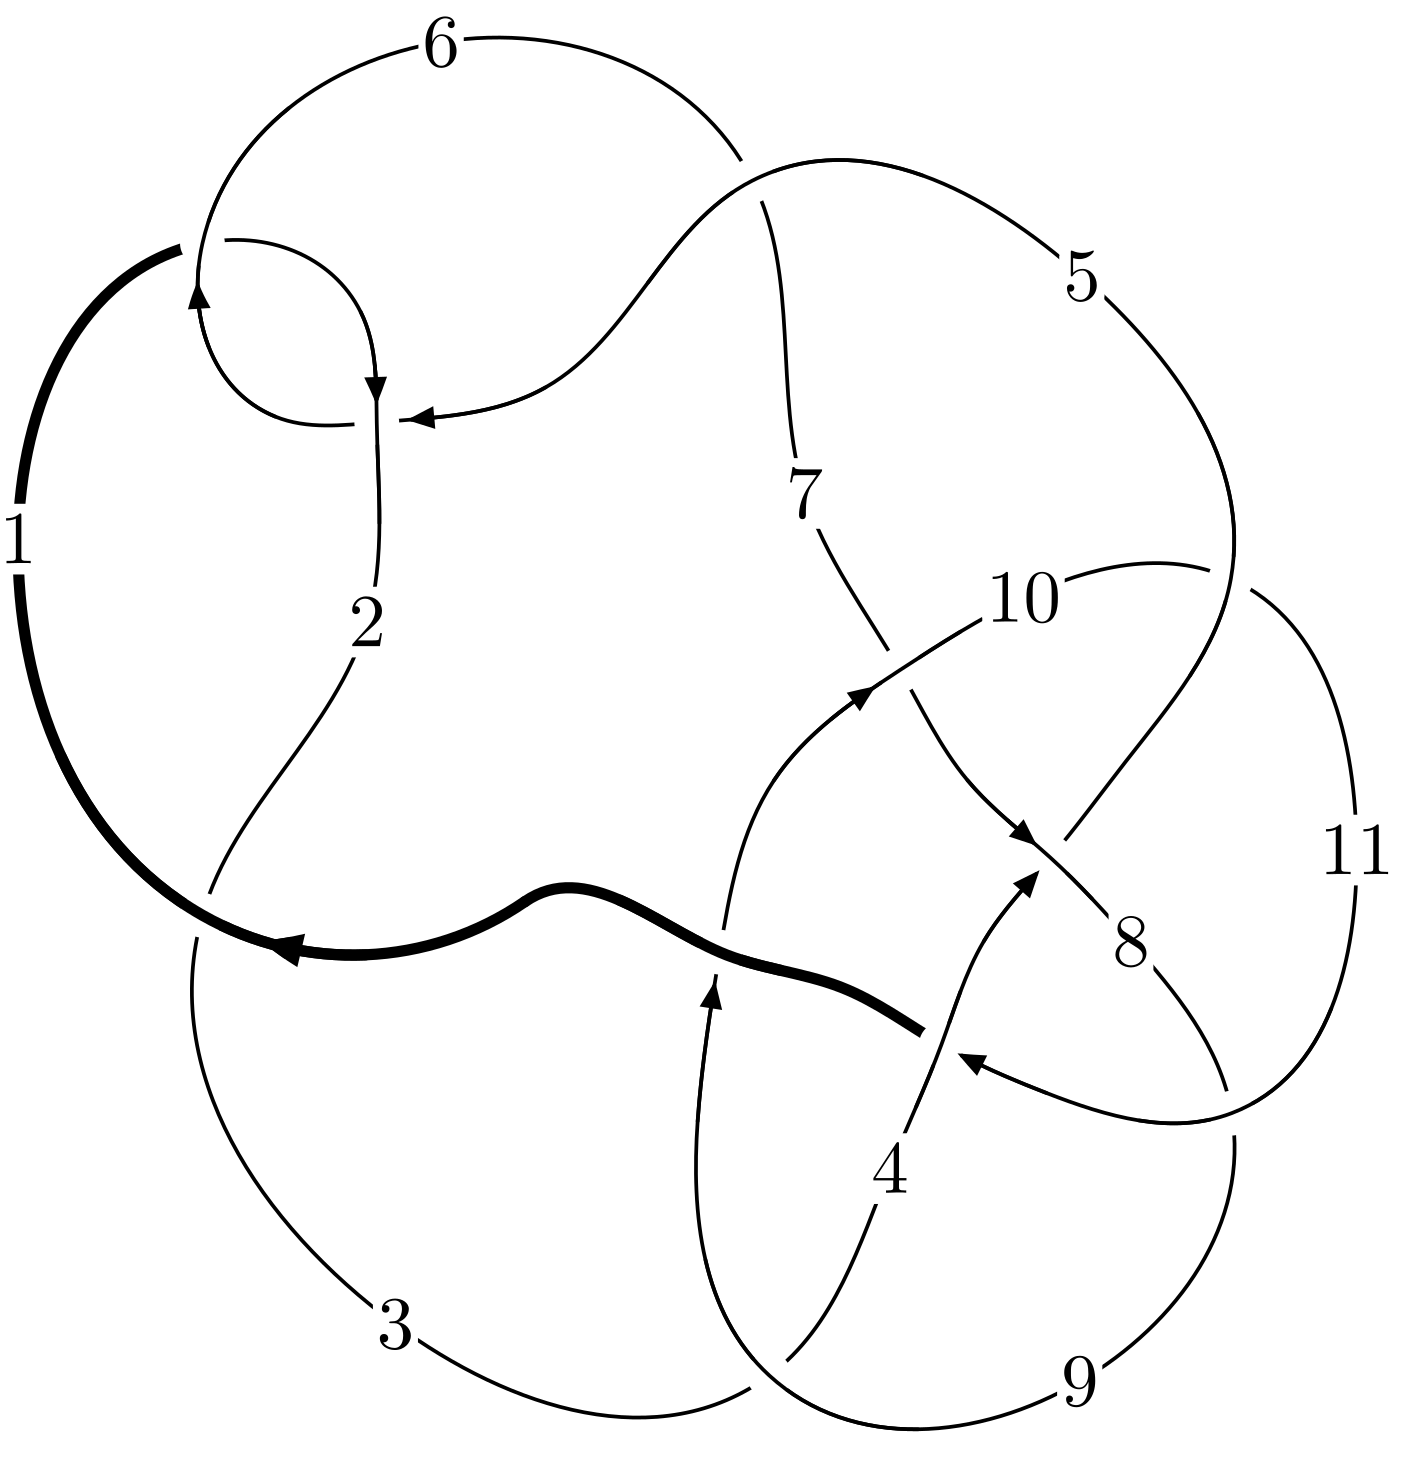
\includegraphics[width=112pt]{../../../GIT/diagram.site/Diagrams/png/739_11n_123.png}\\
\ \ \ A knot diagram\footnotemark}&
\allowdisplaybreaks
\textbf{Linearized knot diagam} \\
\cline{2-2}
 &
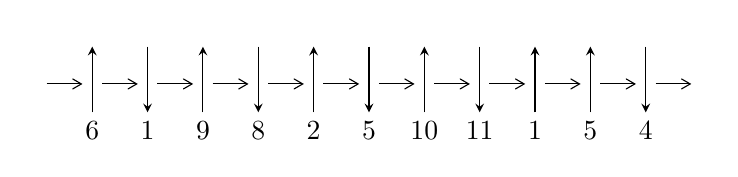
\begin{tikzpicture}[x=20pt, y=17pt]
	% nodes
	\node (C0) at (0, 0) {};
	\node (C1) at (1, 0) {};
	\node (C1U) at (1, +1) {};
	\node (C1D) at (1, -1) {6};

	\node (C2) at (2, 0) {};
	\node (C2U) at (2, +1) {};
	\node (C2D) at (2, -1) {1};

	\node (C3) at (3, 0) {};
	\node (C3U) at (3, +1) {};
	\node (C3D) at (3, -1) {9};

	\node (C4) at (4, 0) {};
	\node (C4U) at (4, +1) {};
	\node (C4D) at (4, -1) {8};

	\node (C5) at (5, 0) {};
	\node (C5U) at (5, +1) {};
	\node (C5D) at (5, -1) {2};

	\node (C6) at (6, 0) {};
	\node (C6U) at (6, +1) {};
	\node (C6D) at (6, -1) {5};

	\node (C7) at (7, 0) {};
	\node (C7U) at (7, +1) {};
	\node (C7D) at (7, -1) {10};

	\node (C8) at (8, 0) {};
	\node (C8U) at (8, +1) {};
	\node (C8D) at (8, -1) {11};

	\node (C9) at (9, 0) {};
	\node (C9U) at (9, +1) {};
	\node (C9D) at (9, -1) {1};

	\node (C10) at (10, 0) {};
	\node (C10U) at (10, +1) {};
	\node (C10D) at (10, -1) {5};

	\node (C11) at (11, 0) {};
	\node (C11U) at (11, +1) {};
	\node (C11D) at (11, -1) {4};
	\node (C12) at (12, 0) {};

	% arrows
	\draw[->,>={angle 60}]
	(C0) edge (C1) (C1) edge (C2) (C2) edge (C3) (C3) edge (C4) (C4) edge (C5) (C5) edge (C6) (C6) edge (C7) (C7) edge (C8) (C8) edge (C9) (C9) edge (C10) (C10) edge (C11) (C11) edge (C12) ;	\draw[->,>=stealth]
	(C1D) edge (C1U) (C2U) edge (C2D) (C3D) edge (C3U) (C4U) edge (C4D) (C5D) edge (C5U) (C6U) edge (C6D) (C7D) edge (C7U) (C8U) edge (C8D) (C9D) edge (C9U) (C10D) edge (C10U) (C11U) edge (C11D) ;
	\end{tikzpicture} \\
\hhline{~~} \\& 
\textbf{Solving Sequence} \\ \cline{2-2} 
 &
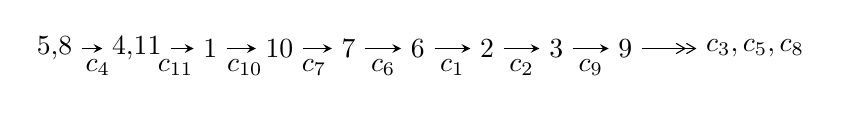
\begin{tikzpicture}[x=25pt, y=7pt]
	% node
	\node (A0) at (-1/8, 0) {5,8};
	\node (A1) at (17/16, 0) {4,11};
	\node (A2) at (17/8, 0) {1};
	\node (A3) at (25/8, 0) {10};
	\node (A4) at (33/8, 0) {7};
	\node (A5) at (41/8, 0) {6};
	\node (A6) at (49/8, 0) {2};
	\node (A7) at (57/8, 0) {3};
	\node (A8) at (65/8, 0) {9};
	\node (C1) at (1/2, -1) {$c_{4}$};
	\node (C2) at (13/8, -1) {$c_{11}$};
	\node (C3) at (21/8, -1) {$c_{10}$};
	\node (C4) at (29/8, -1) {$c_{7}$};
	\node (C5) at (37/8, -1) {$c_{6}$};
	\node (C6) at (45/8, -1) {$c_{1}$};
	\node (C7) at (53/8, -1) {$c_{2}$};
	\node (C8) at (61/8, -1) {$c_{9}$};
	\node (A9) at (10, 0) {$c_{3},c_{5},c_{8}$};

	% edge
	\draw[->,>=stealth]	
	(A0) edge (A1) (A1) edge (A2) (A2) edge (A3) (A3) edge (A4) (A4) edge (A5) (A5) edge (A6) (A6) edge (A7) (A7) edge (A8) ;
	\draw[->>,>={angle 60}]	
	(A8) edge (A9);
\end{tikzpicture} \\ 

\end{tabular} \\

\footnotetext{
The image of knot diagram is generated by the software ``\textbf{Draw programme}" developed by Andrew Bartholomew(\url{http://www.layer8.co.uk/maths/draw/index.htm\#Running-draw}), where we modified some parts for our purpose(\url{https://github.com/CATsTAILs/LinksPainter}).
}\phantom \\ \newline 
\centering \textbf{Ideals for irreducible components\footnotemark of $X_{\text{par}}$} 
 
\begin{align*}
I^u_{1}&=\langle 
-2418 u^{15}-2313 u^{14}+\cdots+1243 b-778,\;-8755 u^{15}-9533 u^{14}+\cdots+1243 a-8595,\\
\phantom{I^u_{1}}&\phantom{= \langle  }u^{16}+u^{15}+5 u^{14}+3 u^{13}+16 u^{12}+7 u^{11}+34 u^{10}+8 u^9+46 u^8-3 u^7+40 u^6-10 u^5+24 u^4-3 u^3+8 u^2+1\rangle \\
I^u_{2}&=\langle 
613651112649 u^{21}+1301363271193 u^{20}+\cdots+2238186198787 b+596588806112,\\
\phantom{I^u_{2}}&\phantom{= \langle  }-1570251208513 u^{21}-3146564850505 u^{20}+\cdots+2238186198787 a-6111907356770,\\
\phantom{I^u_{2}}&\phantom{= \langle  }u^{22}+2 u^{21}+\cdots+3 u+1\rangle \\
I^u_{3}&=\langle 
- u^5+u^4-2 u^3+u^2+b- u,\;-2 u^5+2 u^4-3 u^3+u^2+a-1,\;u^6- u^5+2 u^4- u^3+u^2+1\rangle \\
I^u_{4}&=\langle 
- u^3+u^2+b-3 u+1,\;a,\;u^4- u^3+3 u^2- u+1\rangle \\
\\
\end{align*}
\raggedright * 4 irreducible components of $\dim_{\mathbb{C}}=0$, with total 48 representations.\\
\footnotetext{All coefficients of polynomials are rational numbers. But the coefficients are sometimes approximated in decimal forms when there is not enough margin.}
\newpage
\renewcommand{\arraystretch}{1}
\centering \section*{I. $I^u_{1}= \langle -2418 u^{15}-2313 u^{14}+\cdots+1243 b-778,\;-8755 u^{15}-9533 u^{14}+\cdots+1243 a-8595,\;u^{16}+u^{15}+\cdots+8 u^2+1 \rangle$}
\flushleft \textbf{(i) Arc colorings}\\
\begin{tabular}{m{7pt} m{180pt} m{7pt} m{180pt} }
\flushright $a_{5}=$&$\begin{pmatrix}1\\0\end{pmatrix}$ \\
\flushright $a_{8}=$&$\begin{pmatrix}0\\u\end{pmatrix}$ \\
\flushright $a_{4}=$&$\begin{pmatrix}1\\- u^2\end{pmatrix}$ \\
\flushright $a_{11}=$&$\begin{pmatrix}7.04344 u^{15}+7.66935 u^{14}+\cdots+21.9067 u+6.91472\\1.94529 u^{15}+1.86082 u^{14}+\cdots+8.04344 u+0.625905\end{pmatrix}$ \\
\flushright $a_{1}=$&$\begin{pmatrix}7.04344 u^{15}+7.66935 u^{14}+\cdots+20.9067 u+6.91472\\1.94529 u^{15}+1.86082 u^{14}+\cdots+8.04344 u+0.625905\end{pmatrix}$ \\
\flushright $a_{10}=$&$\begin{pmatrix}5.09815 u^{15}+5.80853 u^{14}+\cdots+13.8632 u+6.28882\\1.94529 u^{15}+1.86082 u^{14}+\cdots+8.04344 u+0.625905\end{pmatrix}$ \\
\flushright $a_{7}=$&$\begin{pmatrix}-3.95414 u^{15}-0.515688 u^{14}+\cdots-25.6541 u+11.7989\\2.08367 u^{15}+2.91874 u^{14}+\cdots+4.22767 u+4.98391\end{pmatrix}$ \\
\flushright $a_{6}=$&$\begin{pmatrix}-1.87047 u^{15}+2.40306 u^{14}+\cdots-21.4264 u+16.7828\\2.08367 u^{15}+2.91874 u^{14}+\cdots+4.22767 u+4.98391\end{pmatrix}$ \\
\flushright $a_{2}=$&$\begin{pmatrix}-4.35800 u^{15}-4.21963 u^{14}+\cdots-16.1569 u-4.81577\\-0.679002 u^{15}+0.390185 u^{14}+\cdots-5.57844 u+3.59212\end{pmatrix}$ \\
\flushright $a_{3}=$&$\begin{pmatrix}-12.5093 u^{15}-14.9574 u^{14}+\cdots-35.6838 u-21.5559\\-4.06436 u^{15}-2.39903 u^{14}+\cdots-18.7136 u+3.08930\end{pmatrix}$ \\
\flushright $a_{9}=$&$\begin{pmatrix}1.72164 u^{15}+6.67418 u^{14}+\cdots-13.6613 u+22.3612\\3.59212 u^{15}+4.27112 u^{14}+\cdots+9.76508 u+5.57844\end{pmatrix}$\\ \flushright $a_{9}=$&$\begin{pmatrix}1.72164 u^{15}+6.67418 u^{14}+\cdots-13.6613 u+22.3612\\3.59212 u^{15}+4.27112 u^{14}+\cdots+9.76508 u+5.57844\end{pmatrix}$\\&\end{tabular}
\flushleft \textbf{(ii) Obstruction class $= -1$}\\~\\
\flushleft \textbf{(iii) Cusp Shapes $= -\frac{7257}{1243} u^{15}-\frac{4223}{1243} u^{14}+\cdots-\frac{16867}{1243} u+\frac{8997}{1243}$}\\~\\
\newpage\renewcommand{\arraystretch}{1}
\flushleft \textbf{(iv) u-Polynomials at the component}\newline \\
\begin{tabular}{m{50pt}|m{274pt}}
Crossings & \hspace{64pt}u-Polynomials at each crossing \\
\hline $$\begin{aligned}c_{1},c_{5}\end{aligned}$$&$\begin{aligned}
&u^{16}-5 u^{15}+\cdots-25 u+4
\end{aligned}$\\
\hline $$\begin{aligned}c_{2},c_{6}\end{aligned}$$&$\begin{aligned}
&u^{16}+11 u^{15}+\cdots+15 u+16
\end{aligned}$\\
\hline $$\begin{aligned}c_{3},c_{10}\end{aligned}$$&$\begin{aligned}
&u^{16}+8 u^{14}+\cdots- u+1
\end{aligned}$\\
\hline $$\begin{aligned}c_{4},c_{11}\end{aligned}$$&$\begin{aligned}
&u^{16}- u^{15}+\cdots+8 u^2+1
\end{aligned}$\\
\hline $$\begin{aligned}c_{7},c_{9}\end{aligned}$$&$\begin{aligned}
&u^{16}-2 u^{15}+\cdots-5 u+1
\end{aligned}$\\
\hline $$\begin{aligned}c_{8}\end{aligned}$$&$\begin{aligned}
&u^{16}-11 u^{15}+\cdots-9 u+2
\end{aligned}$\\
\hline
\end{tabular}\\~\\
\newpage\renewcommand{\arraystretch}{1}
\flushleft \textbf{(v) Riley Polynomials at the component}\newline \\
\begin{tabular}{m{50pt}|m{274pt}}
Crossings & \hspace{64pt}Riley Polynomials at each crossing \\
\hline $$\begin{aligned}c_{1},c_{5}\end{aligned}$$&$\begin{aligned}
&y^{16}+11 y^{15}+\cdots+15 y+16
\end{aligned}$\\
\hline $$\begin{aligned}c_{2},c_{6}\end{aligned}$$&$\begin{aligned}
&y^{16}-9 y^{15}+\cdots+3679 y+256
\end{aligned}$\\
\hline $$\begin{aligned}c_{3},c_{10}\end{aligned}$$&$\begin{aligned}
&y^{16}+16 y^{15}+\cdots+13 y+1
\end{aligned}$\\
\hline $$\begin{aligned}c_{4},c_{11}\end{aligned}$$&$\begin{aligned}
&y^{16}+9 y^{15}+\cdots+16 y+1
\end{aligned}$\\
\hline $$\begin{aligned}c_{7},c_{9}\end{aligned}$$&$\begin{aligned}
&y^{16}+20 y^{15}+\cdots+89 y+1
\end{aligned}$\\
\hline $$\begin{aligned}c_{8}\end{aligned}$$&$\begin{aligned}
&y^{16}-9 y^{15}+\cdots+67 y+4
\end{aligned}$\\
\hline
\end{tabular}\\~\\
\newpage\flushleft \textbf{(vi) Complex Volumes and Cusp Shapes}
$$\begin{array}{c|c|c}  
\text{Solutions to }I^u_{1}& \I (\text{vol} + \sqrt{-1}CS) & \text{Cusp shape}\\
 \hline 
\begin{aligned}
u &= -0.182868 + 1.082360 I \\
a &= -0.245163 + 0.184305 I \\
b &= -0.534837 + 1.195060 I\end{aligned}
 & \phantom{-}0.087550 - 0.115204 I & \phantom{-}2.02768 - 0.43913 I \\ \hline\begin{aligned}
u &= -0.182868 - 1.082360 I \\
a &= -0.245163 - 0.184305 I \\
b &= -0.534837 - 1.195060 I\end{aligned}
 & \phantom{-}0.087550 + 0.115204 I & \phantom{-}2.02768 + 0.43913 I \\ \hline\begin{aligned}
u &= \phantom{-}0.153974 + 1.184900 I \\
a &= \phantom{-}0.067583 - 1.055900 I \\
b &= -0.138027 - 0.297204 I\end{aligned}
 & \phantom{-}4.72589 - 3.00353 I & \phantom{-}9.61260 + 1.22526 I \\ \hline\begin{aligned}
u &= \phantom{-}0.153974 - 1.184900 I \\
a &= \phantom{-}0.067583 + 1.055900 I \\
b &= -0.138027 + 0.297204 I\end{aligned}
 & \phantom{-}4.72589 + 3.00353 I & \phantom{-}9.61260 - 1.22526 I \\ \hline\begin{aligned}
u &= \phantom{-}0.571189 + 0.516899 I \\
a &= \phantom{-}0.465400 + 0.095953 I \\
b &= \phantom{-}0.600357 + 0.236415 I\end{aligned}
 & -0.30256 - 1.83448 I & \phantom{-}0.83977 + 3.70409 I \\ \hline\begin{aligned}
u &= \phantom{-}0.571189 - 0.516899 I \\
a &= \phantom{-}0.465400 - 0.095953 I \\
b &= \phantom{-}0.600357 - 0.236415 I\end{aligned}
 & -0.30256 + 1.83448 I & \phantom{-}0.83977 - 3.70409 I \\ \hline\begin{aligned}
u &= -0.025357 + 0.613269 I \\
a &= -1.140780 + 0.093929 I \\
b &= -0.456590 + 0.613056 I\end{aligned}
 & \phantom{-}0.807041 - 1.112270 I & \phantom{-}4.93277 + 4.22512 I \\ \hline\begin{aligned}
u &= -0.025357 - 0.613269 I \\
a &= -1.140780 - 0.093929 I \\
b &= -0.456590 - 0.613056 I\end{aligned}
 & \phantom{-}0.807041 + 1.112270 I & \phantom{-}4.93277 - 4.22512 I \\ \hline\begin{aligned}
u &= -0.87363 + 1.12508 I \\
a &= -1.102560 - 0.750912 I \\
b &= \phantom{-}0.04840 - 1.41972 I\end{aligned}
 & -9.63409 + 1.32861 I & -2.22452 - 1.49647 I \\ \hline\begin{aligned}
u &= -0.87363 - 1.12508 I \\
a &= -1.102560 + 0.750912 I \\
b &= \phantom{-}0.04840 + 1.41972 I\end{aligned}
 & -9.63409 - 1.32861 I & -2.22452 + 1.49647 I\\
 \hline 
 \end{array}$$\newpage$$\begin{array}{c|c|c}  
\text{Solutions to }I^u_{1}& \I (\text{vol} + \sqrt{-1}CS) & \text{Cusp shape}\\
 \hline 
\begin{aligned}
u &= \phantom{-}0.93365 + 1.17761 I \\
a &= \phantom{-}1.064180 - 0.515654 I \\
b &= \phantom{-}0.34787 - 1.42806 I\end{aligned}
 & -5.07602 - 7.48555 I & \phantom{-}0.37702 + 4.74920 I \\ \hline\begin{aligned}
u &= \phantom{-}0.93365 - 1.17761 I \\
a &= \phantom{-}1.064180 + 0.515654 I \\
b &= \phantom{-}0.34787 + 1.42806 I\end{aligned}
 & -5.07602 + 7.48555 I & \phantom{-}0.37702 - 4.74920 I \\ \hline\begin{aligned}
u &= -0.101130 + 0.483106 I \\
a &= \phantom{-}4.05859 + 0.78880 I \\
b &= \phantom{-}0.727529 + 1.055710 I\end{aligned}
 & -4.12337 + 3.39887 I & \phantom{-}1.84182 + 0.78536 I \\ \hline\begin{aligned}
u &= -0.101130 - 0.483106 I \\
a &= \phantom{-}4.05859 - 0.78880 I \\
b &= \phantom{-}0.727529 - 1.055710 I\end{aligned}
 & -4.12337 - 3.39887 I & \phantom{-}1.84182 - 0.78536 I \\ \hline\begin{aligned}
u &= -0.97583 + 1.17333 I \\
a &= -1.167260 - 0.382800 I \\
b &= -0.59470 - 1.66211 I\end{aligned}
 & -9.5135 + 13.5240 I & -1.40716 - 7.09485 I \\ \hline\begin{aligned}
u &= -0.97583 - 1.17333 I \\
a &= -1.167260 + 0.382800 I \\
b &= -0.59470 + 1.66211 I\end{aligned}
 & -9.5135 - 13.5240 I & -1.40716 + 7.09485 I\\
 \hline 
 \end{array}$$\newpage\newpage\renewcommand{\arraystretch}{1}
\centering \section*{II. $I^u_{2}= \langle 6.14\times10^{11} u^{21}+1.30\times10^{12} u^{20}+\cdots+2.24\times10^{12} b+5.97\times10^{11},\;-1.57\times10^{12} u^{21}-3.15\times10^{12} u^{20}+\cdots+2.24\times10^{12} a-6.11\times10^{12},\;u^{22}+2 u^{21}+\cdots+3 u+1 \rangle$}
\flushleft \textbf{(i) Arc colorings}\\
\begin{tabular}{m{7pt} m{180pt} m{7pt} m{180pt} }
\flushright $a_{5}=$&$\begin{pmatrix}1\\0\end{pmatrix}$ \\
\flushright $a_{8}=$&$\begin{pmatrix}0\\u\end{pmatrix}$ \\
\flushright $a_{4}=$&$\begin{pmatrix}1\\- u^2\end{pmatrix}$ \\
\flushright $a_{11}=$&$\begin{pmatrix}0.701573 u^{21}+1.40585 u^{20}+\cdots+9.05835 u+2.73074\\-0.274173 u^{21}-0.581437 u^{20}+\cdots-5.23195 u-0.266550\end{pmatrix}$ \\
\flushright $a_{1}=$&$\begin{pmatrix}u^{21}+2 u^{20}+\cdots+15 u+3\\-0.298427 u^{21}-0.594145 u^{20}+\cdots-4.94165 u-0.269259\end{pmatrix}$ \\
\flushright $a_{10}=$&$\begin{pmatrix}0.975746 u^{21}+1.98729 u^{20}+\cdots+14.2903 u+2.99729\\-0.274173 u^{21}-0.581437 u^{20}+\cdots-5.23195 u-0.266550\end{pmatrix}$ \\
\flushright $a_{7}=$&$\begin{pmatrix}0.959986 u^{21}+1.89743 u^{20}+\cdots+13.7253 u+3.00284\\-0.378333 u^{21}-0.739672 u^{20}+\cdots-4.23796 u-0.332002\end{pmatrix}$ \\
\flushright $a_{6}=$&$\begin{pmatrix}0.581652 u^{21}+1.15776 u^{20}+\cdots+9.48733 u+2.67084\\-0.378333 u^{21}-0.739672 u^{20}+\cdots-4.23796 u-0.332002\end{pmatrix}$ \\
\flushright $a_{2}=$&$\begin{pmatrix}0.119474 u^{21}+0.251847 u^{20}+\cdots+4.26741 u+2.58228\\-0.0953666 u^{21}-0.241791 u^{20}+\cdots-3.21559 u-0.997831\end{pmatrix}$ \\
\flushright $a_{3}=$&$\begin{pmatrix}0.451476 u^{21}+0.537517 u^{20}+\cdots+7.60383 u-0.659673\\0.0178553 u^{21}+0.0471570 u^{20}+\cdots-1.48034 u+0.254377\end{pmatrix}$ \\
\flushright $a_{9}=$&$\begin{pmatrix}0.391301 u^{21}+0.842507 u^{20}+\cdots+4.87766 u+2.29577\\-0.190351 u^{21}-0.315251 u^{20}+\cdots-2.60967 u-0.375067\end{pmatrix}$\\ \flushright $a_{9}=$&$\begin{pmatrix}0.391301 u^{21}+0.842507 u^{20}+\cdots+4.87766 u+2.29577\\-0.190351 u^{21}-0.315251 u^{20}+\cdots-2.60967 u-0.375067\end{pmatrix}$\\&\end{tabular}
\flushleft \textbf{(ii) Obstruction class $= -1$}\\~\\
\flushleft \textbf{(iii) Cusp Shapes $= -\frac{2340479983939}{2238186198787} u^{21}-\frac{5426028325222}{2238186198787} u^{20}+\cdots-\frac{64839493010449}{2238186198787} u-\frac{12900652043582}{2238186198787}$}\\~\\
\newpage\renewcommand{\arraystretch}{1}
\flushleft \textbf{(iv) u-Polynomials at the component}\newline \\
\begin{tabular}{m{50pt}|m{274pt}}
Crossings & \hspace{64pt}u-Polynomials at each crossing \\
\hline $$\begin{aligned}c_{1},c_{5}\end{aligned}$$&$\begin{aligned}
&(u^{11}+2 u^{10}+\cdots+4 u+1)^{2}
\end{aligned}$\\
\hline $$\begin{aligned}c_{2},c_{6}\end{aligned}$$&$\begin{aligned}
&(u^{11}+8 u^{10}+\cdots-18 u^2-1)^{2}
\end{aligned}$\\
\hline $$\begin{aligned}c_{3},c_{10}\end{aligned}$$&$\begin{aligned}
&u^{22}+10 u^{20}+\cdots+265 u+47
\end{aligned}$\\
\hline $$\begin{aligned}c_{4},c_{11}\end{aligned}$$&$\begin{aligned}
&u^{22}-2 u^{21}+\cdots-3 u+1
\end{aligned}$\\
\hline $$\begin{aligned}c_{7},c_{9}\end{aligned}$$&$\begin{aligned}
&u^{22}+5 u^{21}+\cdots-94 u+53
\end{aligned}$\\
\hline $$\begin{aligned}c_{8}\end{aligned}$$&$\begin{aligned}
&(u^{11}+5 u^{10}+\cdots-10 u-4)^{2}
\end{aligned}$\\
\hline
\end{tabular}\\~\\
\newpage\renewcommand{\arraystretch}{1}
\flushleft \textbf{(v) Riley Polynomials at the component}\newline \\
\begin{tabular}{m{50pt}|m{274pt}}
Crossings & \hspace{64pt}Riley Polynomials at each crossing \\
\hline $$\begin{aligned}c_{1},c_{5}\end{aligned}$$&$\begin{aligned}
&(y^{11}+8 y^{10}+\cdots-18 y^2-1)^{2}
\end{aligned}$\\
\hline $$\begin{aligned}c_{2},c_{6}\end{aligned}$$&$\begin{aligned}
&(y^{11}-8 y^{10}+\cdots-36 y-1)^{2}
\end{aligned}$\\
\hline $$\begin{aligned}c_{3},c_{10}\end{aligned}$$&$\begin{aligned}
&y^{22}+20 y^{21}+\cdots-5647 y+2209
\end{aligned}$\\
\hline $$\begin{aligned}c_{4},c_{11}\end{aligned}$$&$\begin{aligned}
&y^{22}+12 y^{20}+\cdots+21 y+1
\end{aligned}$\\
\hline $$\begin{aligned}c_{7},c_{9}\end{aligned}$$&$\begin{aligned}
&y^{22}+23 y^{21}+\cdots-34700 y+2809
\end{aligned}$\\
\hline $$\begin{aligned}c_{8}\end{aligned}$$&$\begin{aligned}
&(y^{11}-5 y^{10}+\cdots+108 y-16)^{2}
\end{aligned}$\\
\hline
\end{tabular}\\~\\
\newpage\flushleft \textbf{(vi) Complex Volumes and Cusp Shapes}
$$\begin{array}{c|c|c}  
\text{Solutions to }I^u_{2}& \I (\text{vol} + \sqrt{-1}CS) & \text{Cusp shape}\\
 \hline 
\begin{aligned}
u &= \phantom{-}0.459600 + 0.859618 I \\
a &= -1.56146 + 0.19719 I \\
b &= -1.74595 + 0.63036 I\end{aligned}
 & -2.74251 - 5.63735 I & -0.48609 + 8.17754 I \\ \hline\begin{aligned}
u &= \phantom{-}0.459600 - 0.859618 I \\
a &= -1.56146 - 0.19719 I \\
b &= -1.74595 - 0.63036 I\end{aligned}
 & -2.74251 + 5.63735 I & -0.48609 - 8.17754 I \\ \hline\begin{aligned}
u &= -0.670381 + 0.843079 I \\
a &= \phantom{-}1.36153 + 0.63867 I \\
b &= \phantom{-}0.41764 + 1.61796 I\end{aligned}
 & -5.00595 + 2.60776 I & -5.49826 - 2.04245 I \\ \hline\begin{aligned}
u &= -0.670381 - 0.843079 I \\
a &= \phantom{-}1.36153 - 0.63867 I \\
b &= \phantom{-}0.41764 - 1.61796 I\end{aligned}
 & -5.00595 - 2.60776 I & -5.49826 + 2.04245 I \\ \hline\begin{aligned}
u &= \phantom{-}0.783710 + 0.088000 I \\
a &= -1.93047 - 0.70159 I \\
b &= \phantom{-}0.403600 - 0.151320 I\end{aligned}
 & -5.00595 - 2.60776 I & -5.49826 + 2.04245 I \\ \hline\begin{aligned}
u &= \phantom{-}0.783710 - 0.088000 I \\
a &= -1.93047 + 0.70159 I \\
b &= \phantom{-}0.403600 + 0.151320 I\end{aligned}
 & -5.00595 + 2.60776 I & -5.49826 - 2.04245 I \\ \hline\begin{aligned}
u &= \phantom{-}0.816160 + 0.913545 I \\
a &= -1.019150 + 0.057227 I \\
b &= -0.561626 + 0.977866 I\end{aligned}
 & -0.25878 - 3.13682 I & \phantom{-}5.62912 + 1.87495 I \\ \hline\begin{aligned}
u &= \phantom{-}0.816160 - 0.913545 I \\
a &= -1.019150 - 0.057227 I \\
b &= -0.561626 - 0.977866 I\end{aligned}
 & -0.25878 + 3.13682 I & \phantom{-}5.62912 - 1.87495 I \\ \hline\begin{aligned}
u &= -0.475290 + 0.551526 I \\
a &= \phantom{-}1.71279 + 0.12691 I \\
b &= \phantom{-}0.883704 - 0.005644 I\end{aligned}
 & -0.25878 + 3.13682 I & \phantom{-}5.62912 - 1.87495 I \\ \hline\begin{aligned}
u &= -0.475290 - 0.551526 I \\
a &= \phantom{-}1.71279 - 0.12691 I \\
b &= \phantom{-}0.883704 + 0.005644 I\end{aligned}
 & -0.25878 - 3.13682 I & \phantom{-}5.62912 + 1.87495 I\\
 \hline 
 \end{array}$$\newpage$$\begin{array}{c|c|c}  
\text{Solutions to }I^u_{2}& \I (\text{vol} + \sqrt{-1}CS) & \text{Cusp shape}\\
 \hline 
\begin{aligned}
u &= -1.077760 + 0.707508 I \\
a &= \phantom{-}1.108020 - 0.433957 I \\
b &= \phantom{-}0.389001 + 1.117020 I\end{aligned}
 & -2.74251 + 5.63735 I & -0.48609 - 8.17754 I \\ \hline\begin{aligned}
u &= -1.077760 - 0.707508 I \\
a &= \phantom{-}1.108020 + 0.433957 I \\
b &= \phantom{-}0.389001 - 1.117020 I\end{aligned}
 & -2.74251 - 5.63735 I & -0.48609 + 8.17754 I \\ \hline\begin{aligned}
u &= -1.011520 + 0.825413 I \\
a &= -0.633146 - 0.377582 I \\
b &= -0.37963 - 1.79002 I\end{aligned}
 & -10.59450 + 5.64581 I & -3.10897 - 3.66343 I \\ \hline\begin{aligned}
u &= -1.011520 - 0.825413 I \\
a &= -0.633146 + 0.377582 I \\
b &= -0.37963 + 1.79002 I\end{aligned}
 & -10.59450 - 5.64581 I & -3.10897 + 3.66343 I \\ \hline\begin{aligned}
u &= \phantom{-}1.133190 + 0.778692 I \\
a &= \phantom{-}0.533769 - 0.366790 I \\
b &= \phantom{-}0.12411 - 1.47210 I\end{aligned}
 & -6.33840\phantom{ +0.000000I} &                  -6
-1.167441 + 0. 10   I\phantom{ +0.000000I} \\ \hline\begin{aligned}
u &= \phantom{-}1.133190 - 0.778692 I \\
a &= \phantom{-}0.533769 + 0.366790 I \\
b &= \phantom{-}0.12411 + 1.47210 I\end{aligned}
 & -6.33840\phantom{ +0.000000I} &                  -6
-1.167441 + 0. 10   I\phantom{ +0.000000I} \\ \hline\begin{aligned}
u &= \phantom{-}0.35734 + 1.44486 I \\
a &= -0.249751 + 0.405356 I \\
b &= -0.159367 + 0.805498 I\end{aligned}
 & \phantom{-}1.20928 - 2.43685 I & -2.45208 + 7.14380 I \\ \hline\begin{aligned}
u &= \phantom{-}0.35734 - 1.44486 I \\
a &= -0.249751 - 0.405356 I \\
b &= -0.159367 - 0.805498 I\end{aligned}
 & \phantom{-}1.20928 + 2.43685 I & -2.45208 - 7.14380 I \\ \hline\begin{aligned}
u &= -1.22659 + 0.86184 I \\
a &= -0.465716 - 0.441913 I \\
b &= \phantom{-}0.27756 - 1.47343 I\end{aligned}
 & -10.59450 - 5.64581 I & -3.10897 + 3.66343 I \\ \hline\begin{aligned}
u &= -1.22659 - 0.86184 I \\
a &= -0.465716 + 0.441913 I \\
b &= \phantom{-}0.27756 + 1.47343 I\end{aligned}
 & -10.59450 + 5.64581 I & -3.10897 - 3.66343 I\\
 \hline 
 \end{array}$$\newpage$$\begin{array}{c|c|c}  
\text{Solutions to }I^u_{2}& \I (\text{vol} + \sqrt{-1}CS) & \text{Cusp shape}\\
 \hline 
\begin{aligned}
u &= -0.088447 + 0.246861 I \\
a &= \phantom{-}1.64359 + 2.14516 I \\
b &= \phantom{-}0.350965 - 1.259140 I\end{aligned}
 & \phantom{-}1.20928 + 2.43685 I & -2.45208 - 7.14380 I \\ \hline\begin{aligned}
u &= -0.088447 - 0.246861 I \\
a &= \phantom{-}1.64359 - 2.14516 I \\
b &= \phantom{-}0.350965 + 1.259140 I\end{aligned}
 & \phantom{-}1.20928 - 2.43685 I & -2.45208 + 7.14380 I\\
 \hline 
 \end{array}$$\newpage\newpage\renewcommand{\arraystretch}{1}
\centering \section*{III. $I^u_{3}= \langle - u^5+u^4-2 u^3+u^2+b- u,\;-2 u^5+2 u^4-3 u^3+u^2+a-1,\;u^6- u^5+2 u^4- u^3+u^2+1 \rangle$}
\flushleft \textbf{(i) Arc colorings}\\
\begin{tabular}{m{7pt} m{180pt} m{7pt} m{180pt} }
\flushright $a_{5}=$&$\begin{pmatrix}1\\0\end{pmatrix}$ \\
\flushright $a_{8}=$&$\begin{pmatrix}0\\u\end{pmatrix}$ \\
\flushright $a_{4}=$&$\begin{pmatrix}1\\- u^2\end{pmatrix}$ \\
\flushright $a_{11}=$&$\begin{pmatrix}2 u^5-2 u^4+3 u^3- u^2+1\\u^5- u^4+2 u^3- u^2+u\end{pmatrix}$ \\
\flushright $a_{1}=$&$\begin{pmatrix}2 u^5-2 u^4+3 u^3- u^2+u+1\\u^5- u^4+u^3- u^2+u\end{pmatrix}$ \\
\flushright $a_{10}=$&$\begin{pmatrix}u^5- u^4+u^3- u+1\\u^5- u^4+2 u^3- u^2+u\end{pmatrix}$ \\
\flushright $a_{7}=$&$\begin{pmatrix}- u^5+2 u^4-4 u^3+4 u^2-3 u+1\\u^5- u^4+u^3+1\end{pmatrix}$ \\
\flushright $a_{6}=$&$\begin{pmatrix}u^4-3 u^3+4 u^2-3 u+2\\u^5- u^4+u^3+1\end{pmatrix}$ \\
\flushright $a_{2}=$&$\begin{pmatrix}- u^5+u^4-2 u^3+u^2-2\\- u^3+u^2- u\end{pmatrix}$ \\
\flushright $a_{3}=$&$\begin{pmatrix}-3 u^5+5 u^4-7 u^3+3 u^2-3\\- u^5+3 u^4-4 u^3+3 u^2-2 u+1\end{pmatrix}$ \\
\flushright $a_{9}=$&$\begin{pmatrix}2 u^5- u^4+3 u^2-4 u+3\\2 u^5-2 u^4+3 u^3- u^2+u+1\end{pmatrix}$\\ \flushright $a_{9}=$&$\begin{pmatrix}2 u^5- u^4+3 u^2-4 u+3\\2 u^5-2 u^4+3 u^3- u^2+u+1\end{pmatrix}$\\&\end{tabular}
\flushleft \textbf{(ii) Obstruction class $= 1$}\\~\\
\flushleft \textbf{(iii) Cusp Shapes $= 6 u^4-7 u^3+12 u^2-4 u+2$}\\~\\
\newpage\renewcommand{\arraystretch}{1}
\flushleft \textbf{(iv) u-Polynomials at the component}\newline \\
\begin{tabular}{m{50pt}|m{274pt}}
Crossings & \hspace{64pt}u-Polynomials at each crossing \\
\hline $$\begin{aligned}c_{1}\end{aligned}$$&$\begin{aligned}
&u^6-2 u^5+4 u^4-4 u^3+4 u^2- u+1
\end{aligned}$\\
\hline $$\begin{aligned}c_{2},c_{6}\end{aligned}$$&$\begin{aligned}
&u^6+4 u^5+8 u^4+14 u^3+16 u^2+7 u+1
\end{aligned}$\\
\hline $$\begin{aligned}c_{3},c_{10}\end{aligned}$$&$\begin{aligned}
&u^6+u^4- u^3+2 u^2- u+1
\end{aligned}$\\
\hline $$\begin{aligned}c_{4},c_{11}\end{aligned}$$&$\begin{aligned}
&u^6- u^5+2 u^4- u^3+u^2+1
\end{aligned}$\\
\hline $$\begin{aligned}c_{5}\end{aligned}$$&$\begin{aligned}
&u^6+2 u^5+4 u^4+4 u^3+4 u^2+u+1
\end{aligned}$\\
\hline $$\begin{aligned}c_{7},c_{9}\end{aligned}$$&$\begin{aligned}
&u^6-2 u^5+5 u^4-5 u^3+4 u^2-3 u+1
\end{aligned}$\\
\hline $$\begin{aligned}c_{8}\end{aligned}$$&$\begin{aligned}
&u^6-8 u^5+30 u^4-65 u^3+84 u^2-62 u+21
\end{aligned}$\\
\hline
\end{tabular}\\~\\
\newpage\renewcommand{\arraystretch}{1}
\flushleft \textbf{(v) Riley Polynomials at the component}\newline \\
\begin{tabular}{m{50pt}|m{274pt}}
Crossings & \hspace{64pt}Riley Polynomials at each crossing \\
\hline $$\begin{aligned}c_{1},c_{5}\end{aligned}$$&$\begin{aligned}
&y^6+4 y^5+8 y^4+14 y^3+16 y^2+7 y+1
\end{aligned}$\\
\hline $$\begin{aligned}c_{2},c_{6}\end{aligned}$$&$\begin{aligned}
&y^6-16 y^4+6 y^3+76 y^2-17 y+1
\end{aligned}$\\
\hline $$\begin{aligned}c_{3},c_{10}\end{aligned}$$&$\begin{aligned}
&y^6+2 y^5+5 y^4+5 y^3+4 y^2+3 y+1
\end{aligned}$\\
\hline $$\begin{aligned}c_{4},c_{11}\end{aligned}$$&$\begin{aligned}
&y^6+3 y^5+4 y^4+5 y^3+5 y^2+2 y+1
\end{aligned}$\\
\hline $$\begin{aligned}c_{7},c_{9}\end{aligned}$$&$\begin{aligned}
&y^6+6 y^5+13 y^4+5 y^3-4 y^2- y+1
\end{aligned}$\\
\hline $$\begin{aligned}c_{8}\end{aligned}$$&$\begin{aligned}
&y^6-4 y^5+28 y^4-135 y^3+256 y^2-316 y+441
\end{aligned}$\\
\hline
\end{tabular}\\~\\
\newpage\flushleft \textbf{(vi) Complex Volumes and Cusp Shapes}
$$\begin{array}{c|c|c}  
\text{Solutions to }I^u_{3}& \I (\text{vol} + \sqrt{-1}CS) & \text{Cusp shape}\\
 \hline 
\begin{aligned}
u &= \phantom{-}0.800501 + 0.710292 I \\
a &= -1.163950 - 0.050182 I \\
b &= -0.698934 + 0.620170 I\end{aligned}
 & -1.27956 - 3.69612 I & -2.32375 + 5.61497 I \\ \hline\begin{aligned}
u &= \phantom{-}0.800501 - 0.710292 I \\
a &= -1.163950 + 0.050182 I \\
b &= -0.698934 - 0.620170 I\end{aligned}
 & -1.27956 + 3.69612 I & -2.32375 - 5.61497 I \\ \hline\begin{aligned}
u &= \phantom{-}0.155981 + 1.227730 I \\
a &= -0.297083 + 1.291660 I \\
b &= -0.101839 + 0.801573 I\end{aligned}
 & \phantom{-}3.99825 - 3.41127 I & \phantom{-}0.80640 + 5.19600 I \\ \hline\begin{aligned}
u &= \phantom{-}0.155981 - 1.227730 I \\
a &= -0.297083 - 1.291660 I \\
b &= -0.101839 - 0.801573 I\end{aligned}
 & \phantom{-}3.99825 + 3.41127 I & \phantom{-}0.80640 - 5.19600 I \\ \hline\begin{aligned}
u &= -0.456483 + 0.601395 I \\
a &= \phantom{-}2.96104 + 0.19968 I \\
b &= \phantom{-}0.800773 + 1.054980 I\end{aligned}
 & -4.36362 + 4.05299 I & -2.48265 - 9.09326 I \\ \hline\begin{aligned}
u &= -0.456483 - 0.601395 I \\
a &= \phantom{-}2.96104 - 0.19968 I \\
b &= \phantom{-}0.800773 - 1.054980 I\end{aligned}
 & -4.36362 - 4.05299 I & -2.48265 + 9.09326 I\\
 \hline 
 \end{array}$$\newpage\newpage\renewcommand{\arraystretch}{1}
\centering \section*{IV. $I^u_{4}= \langle - u^3+u^2+b-3 u+1,\;a,\;u^4- u^3+3 u^2- u+1 \rangle$}
\flushleft \textbf{(i) Arc colorings}\\
\begin{tabular}{m{7pt} m{180pt} m{7pt} m{180pt} }
\flushright $a_{5}=$&$\begin{pmatrix}1\\0\end{pmatrix}$ \\
\flushright $a_{8}=$&$\begin{pmatrix}0\\u\end{pmatrix}$ \\
\flushright $a_{4}=$&$\begin{pmatrix}1\\- u^2\end{pmatrix}$ \\
\flushright $a_{11}=$&$\begin{pmatrix}0\\u^3- u^2+3 u-1\end{pmatrix}$ \\
\flushright $a_{1}=$&$\begin{pmatrix}- u^3+u^2-3 u+1\\u^3- u^2+2 u-1\end{pmatrix}$ \\
\flushright $a_{10}=$&$\begin{pmatrix}- u^3+u^2-3 u+1\\u^3- u^2+3 u-1\end{pmatrix}$ \\
\flushright $a_{7}=$&$\begin{pmatrix}u^3- u^2+3 u-1\\- u^3+u^2-2 u+1\end{pmatrix}$ \\
\flushright $a_{6}=$&$\begin{pmatrix}u\\- u^3+u^2-2 u+1\end{pmatrix}$ \\
\flushright $a_{2}=$&$\begin{pmatrix}- u^3-2 u\\u^3- u^2+2 u\end{pmatrix}$ \\
\flushright $a_{3}=$&$\begin{pmatrix}1\\0\end{pmatrix}$ \\
\flushright $a_{9}=$&$\begin{pmatrix}0\\u\end{pmatrix}$\\ \flushright $a_{9}=$&$\begin{pmatrix}0\\u\end{pmatrix}$\\&\end{tabular}
\flushleft \textbf{(ii) Obstruction class $= 1$}\\~\\
\flushleft \textbf{(iii) Cusp Shapes $= u^3- u^2+2 u+7$}\\~\\
\newpage\renewcommand{\arraystretch}{1}
\flushleft \textbf{(iv) u-Polynomials at the component}\newline \\
\begin{tabular}{m{50pt}|m{274pt}}
Crossings & \hspace{64pt}u-Polynomials at each crossing \\
\hline $$\begin{aligned}c_{1},c_{2},c_{6}\end{aligned}$$&$\begin{aligned}
&(u^2+u+1)^2
\end{aligned}$\\
\hline $$\begin{aligned}c_{3},c_{4},c_{10}\\c_{11}\end{aligned}$$&$\begin{aligned}
&u^4- u^3+3 u^2- u+1
\end{aligned}$\\
\hline $$\begin{aligned}c_{5}\end{aligned}$$&$\begin{aligned}
&(u^2- u+1)^2
\end{aligned}$\\
\hline $$\begin{aligned}c_{7},c_{9}\end{aligned}$$&$\begin{aligned}
&(u+1)^4
\end{aligned}$\\
\hline $$\begin{aligned}c_{8}\end{aligned}$$&$\begin{aligned}
&u^4
\end{aligned}$\\
\hline
\end{tabular}\\~\\
\newpage\renewcommand{\arraystretch}{1}
\flushleft \textbf{(v) Riley Polynomials at the component}\newline \\
\begin{tabular}{m{50pt}|m{274pt}}
Crossings & \hspace{64pt}Riley Polynomials at each crossing \\
\hline $$\begin{aligned}c_{1},c_{2},c_{5}\\c_{6}\end{aligned}$$&$\begin{aligned}
&(y^2+y+1)^2
\end{aligned}$\\
\hline $$\begin{aligned}c_{3},c_{4},c_{10}\\c_{11}\end{aligned}$$&$\begin{aligned}
&y^4+5 y^3+9 y^2+5 y+1
\end{aligned}$\\
\hline $$\begin{aligned}c_{7},c_{9}\end{aligned}$$&$\begin{aligned}
&(y-1)^4
\end{aligned}$\\
\hline $$\begin{aligned}c_{8}\end{aligned}$$&$\begin{aligned}
&y^4
\end{aligned}$\\
\hline
\end{tabular}\\~\\
\newpage\flushleft \textbf{(vi) Complex Volumes and Cusp Shapes}
$$\begin{array}{c|c|c}  
\text{Solutions to }I^u_{4}& \I (\text{vol} + \sqrt{-1}CS) & \text{Cusp shape}\\
 \hline 
\begin{aligned}
u &= \phantom{-}0.148403 + 0.632502 I \\
a &= \phantom{-0.000000 } 0 \\
b &= -0.35160 + 1.49853 I\end{aligned}
 & \phantom{-}1.64493 + 2.02988 I & \phantom{-}7.50000 + 0.86603 I \\ \hline\begin{aligned}
u &= \phantom{-}0.148403 - 0.632502 I \\
a &= \phantom{-0.000000 } 0 \\
b &= -0.35160 - 1.49853 I\end{aligned}
 & \phantom{-}1.64493 - 2.02988 I & \phantom{-}7.50000 - 0.86603 I \\ \hline\begin{aligned}
u &= \phantom{-}0.35160 + 1.49853 I \\
a &= \phantom{-0.000000 } 0 \\
b &= -0.148403 + 0.632502 I\end{aligned}
 & \phantom{-}1.64493 - 2.02988 I & \phantom{-}7.50000 - 0.86603 I \\ \hline\begin{aligned}
u &= \phantom{-}0.35160 - 1.49853 I \\
a &= \phantom{-0.000000 } 0 \\
b &= -0.148403 - 0.632502 I\end{aligned}
 & \phantom{-}1.64493 + 2.02988 I & \phantom{-}7.50000 + 0.86603 I\\
 \hline 
 \end{array}$$\newpage
\newpage\renewcommand{\arraystretch}{1}
\centering \section*{ V. u-Polynomials}
\begin{tabular}{m{50pt}|m{274pt}}
Crossings & \hspace{64pt}u-Polynomials at each crossing \\
\hline $$\begin{aligned}c_{1}\end{aligned}$$&$\begin{aligned}
&(u^2+u+1)^2(u^6-2 u^5+4 u^4-4 u^3+4 u^2- u+1)\\
&\cdot((u^{11}+2 u^{10}+\cdots+4 u+1)^{2})(u^{16}-5 u^{15}+\cdots-25 u+4)
\end{aligned}$\\
\hline $$\begin{aligned}c_{2},c_{6}\end{aligned}$$&$\begin{aligned}
&(u^2+u+1)^2(u^6+4 u^5+8 u^4+14 u^3+16 u^2+7 u+1)\\
&\cdot((u^{11}+8 u^{10}+\cdots-18 u^2-1)^{2})(u^{16}+11 u^{15}+\cdots+15 u+16)
\end{aligned}$\\
\hline $$\begin{aligned}c_{3},c_{10}\end{aligned}$$&$\begin{aligned}
&(u^4- u^3+3 u^2- u+1)(u^6+u^4- u^3+2 u^2- u+1)\\
&\cdot(u^{16}+8 u^{14}+\cdots- u+1)(u^{22}+10 u^{20}+\cdots+265 u+47)
\end{aligned}$\\
\hline $$\begin{aligned}c_{4},c_{11}\end{aligned}$$&$\begin{aligned}
&(u^4- u^3+3 u^2- u+1)(u^6- u^5+2 u^4- u^3+u^2+1)\\
&\cdot(u^{16}- u^{15}+\cdots+8 u^2+1)(u^{22}-2 u^{21}+\cdots-3 u+1)
\end{aligned}$\\
\hline $$\begin{aligned}c_{5}\end{aligned}$$&$\begin{aligned}
&(u^2- u+1)^2(u^6+2 u^5+4 u^4+4 u^3+4 u^2+u+1)\\
&\cdot((u^{11}+2 u^{10}+\cdots+4 u+1)^{2})(u^{16}-5 u^{15}+\cdots-25 u+4)
\end{aligned}$\\
\hline $$\begin{aligned}c_{7},c_{9}\end{aligned}$$&$\begin{aligned}
&(u+1)^4(u^6-2 u^5+5 u^4-5 u^3+4 u^2-3 u+1)\\
&\cdot(u^{16}-2 u^{15}+\cdots-5 u+1)(u^{22}+5 u^{21}+\cdots-94 u+53)
\end{aligned}$\\
\hline $$\begin{aligned}c_{8}\end{aligned}$$&$\begin{aligned}
&u^4(u^6-8 u^5+30 u^4-65 u^3+84 u^2-62 u+21)\\
&\cdot((u^{11}+5 u^{10}+\cdots-10 u-4)^{2})(u^{16}-11 u^{15}+\cdots-9 u+2)
\end{aligned}$\\
\hline
\end{tabular}\newpage\renewcommand{\arraystretch}{1}
\centering \section*{ VI. Riley Polynomials}
\begin{tabular}{m{50pt}|m{274pt}}
Crossings & \hspace{64pt}Riley Polynomials at each crossing \\
\hline $$\begin{aligned}c_{1},c_{5}\end{aligned}$$&$\begin{aligned}
&(y^2+y+1)^2(y^6+4 y^5+8 y^4+14 y^3+16 y^2+7 y+1)\\
&\cdot((y^{11}+8 y^{10}+\cdots-18 y^2-1)^{2})(y^{16}+11 y^{15}+\cdots+15 y+16)
\end{aligned}$\\
\hline $$\begin{aligned}c_{2},c_{6}\end{aligned}$$&$\begin{aligned}
&(y^2+y+1)^2(y^6-16 y^4+6 y^3+76 y^2-17 y+1)\\
&\cdot((y^{11}-8 y^{10}+\cdots-36 y-1)^{2})(y^{16}-9 y^{15}+\cdots+3679 y+256)
\end{aligned}$\\
\hline $$\begin{aligned}c_{3},c_{10}\end{aligned}$$&$\begin{aligned}
&(y^4+5 y^3+9 y^2+5 y+1)(y^6+2 y^5+5 y^4+5 y^3+4 y^2+3 y+1)\\
&\cdot(y^{16}+16 y^{15}+\cdots+13 y+1)(y^{22}+20 y^{21}+\cdots-5647 y+2209)
\end{aligned}$\\
\hline $$\begin{aligned}c_{4},c_{11}\end{aligned}$$&$\begin{aligned}
&(y^4+5 y^3+9 y^2+5 y+1)(y^6+3 y^5+4 y^4+5 y^3+5 y^2+2 y+1)\\
&\cdot(y^{16}+9 y^{15}+\cdots+16 y+1)(y^{22}+12 y^{20}+\cdots+21 y+1)
\end{aligned}$\\
\hline $$\begin{aligned}c_{7},c_{9}\end{aligned}$$&$\begin{aligned}
&(y-1)^4(y^6+6 y^5+13 y^4+5 y^3-4 y^2- y+1)\\
&\cdot(y^{16}+20 y^{15}+\cdots+89 y+1)(y^{22}+23 y^{21}+\cdots-34700 y+2809)
\end{aligned}$\\
\hline $$\begin{aligned}c_{8}\end{aligned}$$&$\begin{aligned}
&y^4(y^6-4 y^5+28 y^4-135 y^3+256 y^2-316 y+441)\\
&\cdot((y^{11}-5 y^{10}+\cdots+108 y-16)^{2})(y^{16}-9 y^{15}+\cdots+67 y+4)
\end{aligned}$\\
\hline
\end{tabular}
\vskip 2pc
\end{document}